\section{Part I: Reconstructor Nonlinearity Ablation (\texttt{RQ2})}
\label{sec:rq2}

In our first experimental campaign (\texttt{RQ2}), we hold the dynamics architecture $\NNdyn$, data splits, loss functions, and two-stage Adam+BFGS optimizer schedule fixed, and systematically replace $\NNrec$ across the hierarchy $\mathrm{L0} \to \mathrm{L1} \to \mathrm{L2} \to \mathrm{L3}$ under both frozen-latent ($\mathrm{R1}$) and end-to-end ($\mathrm{R2}$) training regimes. Across the three PDE benchmarks, the sweep covers $d_s \in \{1,2,3,5\}$ and $K \in \{d_s, 3, 5, 9, 17, 33, 65\}$ in Case~A (348 runs), $d_s \in \{1,5,10\}$ and $K \in \{d_s, 3, 5, 9, 17\}$ in Case~B (195 runs), and $d_s \in \{1,2,3,5,12\}$ and $K \in \{d_s, 5, 17, 33\}$ in Case~C (273 runs), with 3 random seeds $\{0,1,2\}$ per configuration, totalling \textbf{816 trained models}.

\subsection{Experimental Protocol and Statistical Reporting}

In \texttt{RQ2}, training uses Adam with learning rate $10^{-2}$ followed by \texttt{scipy} BFGS: 50 Adam + 150 BFGS epochs in Case~A (matching the original notebook), and 200 Adam + 500 BFGS epochs in Cases~B and~C (a reduced budget adopted so that the 468 runs of Cases~B and~C could be completed on a single workstation; the full $10{,}000$-iteration BFGS regime is the subject of Part~II in Section~\ref{sec:rq2bis}). For every procedure (a pair of variant $\mathrm{L}m$ and regime $\mathrm{R}j$), the best configuration $(d_s, K)$ is selected strictly on the \textbf{validation set} median NRMSE; the test set is never used for model selection. Because three seeds do not permit parametric hypothesis tests with statistical power below $p = 0.10$ (the minimum two-sided permutation $p$-value of two disjoint triples is $2/\binom{6}{3} = 0.10$), we report the median across the three seeds, the full range $[\min, \max]$, the ratio of medians relative to $\mathrm{L0}$, and whether the three seeds of a procedure are \emph{completely separated} from the three seeds of $\mathrm{L0}$.

\subsection{Case A Results: Smooth Periodic Dynamics and Curved Latent Coordinates}

Table~\ref{tab:rq2_caseA} summarises the validation-selected best configurations, the $d_s$-sweep of $\mathrm{L0}$ and $\mathrm{L1}$, and the $K$-sweep of $\mathrm{L2}$ and $\mathrm{L3}$ at $d_s = 3$ for Case~A.

\begin{table}[!htbp]
\centering
\caption{Case A (\texttt{ADR-1b}) results in \texttt{RQ2} (50 Adam + 150 BFGS epochs). \textbf{Top:} best configuration of each procedure selected on validation NRMSE (median and $[\min,\max]$ over 3 seeds). \textbf{Bottom:} test NRMSE across the modal truncation sweep $K$ at $d_s = 3$, together with the parameter-matched hidden width $w_g$ of $\mathrm{L3}$.}
\label{tab:rq2_caseA}
\small\resizebox{\textwidth}{!}{%

\begin{tabular}{@{}lrrrlrrlrr@{}}
\toprule
\textbf{Procedure} & $d_s$ & $K$ & $P_{\mathrm{rec}}$ & \textbf{Test NRMSE $[\min, \max]$} & $1-\rho$ & $\varepsilon_{\mathrm{total}}$ & \textbf{Ratio to L0} & \textbf{Separated} & \textbf{Train [s] / Infer [ms]} \\
\midrule
$\mathrm{L0}$ (R2) & $5$ & -- & $113$ & $2.26\cdot 10^{-2}$ $[1.96, 2.65]\cdot 10^{-2}$ & $9.05\cdot 10^{-3}$ & $0.134$ & $1.00$ & -- & $14.3$ / $14.7$ \\
$\mathrm{L1}$-R1 & $1$ & $1$ & $0$ & $1.68\cdot 10^{-1}$ $[1.64, 1.80]\cdot 10^{-1}$ & $6.30\cdot 10^{-1}$ & $0.995$ & $7.41$ & yes (worse) & $0.0$ / $0.3$ \\
$\mathrm{L1}$-R2 & $3$ & $3$ & $0$ & $2.85\cdot 10^{-2}$ $[2.57, 2.88]\cdot 10^{-2}$ & $1.35\cdot 10^{-2}$ & $0.169$ & $1.26$ & no & $3.8$ / $1.7$ \\
$\mathrm{L2}$-R1 & $5$ & $3$ & $18$ & $1.02\cdot 10^{-1}$ $[1.01, 1.02]\cdot 10^{-1}$ & $2.02\cdot 10^{-1}$ & $0.607$ & $4.52$ & yes (worse) & $0.0$ / $1.0$ \\
$\mathbf{L2}$\textbf{-R2} & $\mathbf{3}$ & $\mathbf{5}$ & $\mathbf{20}$ & $\mathbf{9.72\cdot 10^{-3}}$ $[9.26\cdot 10^{-3}, 1.36\cdot 10^{-2}]$ & $\mathbf{1.65\cdot 10^{-3}}$ & $\mathbf{0.058}$ & $\mathbf{0.43}$ & \textbf{yes (better)} & $\mathbf{4.1}$ / $\mathbf{1.8}$ \\
$\mathrm{L3}$-R1 & $3$ & $3$ & $87$ & $2.30\cdot 10^{-2}$ $[2.23, 2.42]\cdot 10^{-2}$ & $9.32\cdot 10^{-3}$ & $0.136$ & $1.01$ & no & $2.0$ / $3.6$ \\
$\mathrm{L3}$-R2 & $3$ & $17$ & $92$ & $1.18\cdot 10^{-2}$ $[1.09, 1.90]\cdot 10^{-2}$ & $2.43\cdot 10^{-3}$ & $0.070$ & $0.52$ & yes (better) & $5.5$ / $3.6$ \\
\bottomrule
\end{tabular}
}

\vspace{0.6em}\resizebox{\textwidth}{!}{%

\begin{tabular}{@{}lcccccc@{}}
\toprule
\textbf{K-Sweep at $d_s = 3$} & $K = 3$ & $K = 5$ & $K = 9$ & $K = 17$ & $K = 33$ & $K = 65$ \\
\midrule
$\mathrm{L2}$-R2 (end-to-end affine) & $1.32\cdot 10^{-2}$ & $9.72\cdot 10^{-3}$ & $1.03\cdot 10^{-2}$ & $1.36\cdot 10^{-2}$ & $1.20\cdot 10^{-2}$ & $1.20\cdot 10^{-2}$ \\
$\mathrm{L2}$-R1 (frozen $\mathrm{L0}$ latents) & $1.04\cdot 10^{-1}$ & $1.04\cdot 10^{-1}$ & $1.04\cdot 10^{-1}$ & $1.04\cdot 10^{-1}$ & $1.04\cdot 10^{-1}$ & $1.04\cdot 10^{-1}$ \\
$\mathrm{L3}$-R2 (end-to-end MLP) & $1.65\cdot 10^{-2}$ & $1.48\cdot 10^{-2}$ & $1.98\cdot 10^{-2}$ & $1.18\cdot 10^{-2}$ & $9.55\cdot 10^{-2}$ & $9.55\cdot 10^{-2}$ \\
$\mathrm{L3}$-R1 (frozen $\mathrm{L0}$ latents) & $2.30\cdot 10^{-2}$ & $2.32\cdot 10^{-2}$ & $2.45\cdot 10^{-2}$ & $4.23\cdot 10^{-2}$ & $1.07\cdot 10^{-1}$ & $1.07\cdot 10^{-1}$ \\
Matched hidden width $w_g$ of $\mathrm{L3}$ & $6$ & $5$ & $4$ & $3$ & $1$ & $1$ \\
\bottomrule
\end{tabular}
}
\end{table}

Four key findings emerge from Case~A:
\begin{enumerate}[leftmargin=2em]
  \item \textbf{End-to-end affine reconstruction ($\mathrm{L2}$-R2) beats $\mathrm{L0}$ by $2.3\times$ with $5.6\times$ fewer parameters:} Once $K \ge 3$ includes $\cos(\pi x)$ and $\sin(\pi x)$, $\mathrm{L2}$-R2 reaches $\NRMSE = 9.72\cdot 10^{-3}$ ($P_{\mathrm{rec}} = 20$), compared with $2.26\cdot 10^{-2}$ for $\mathrm{L0}$ ($P_{\mathrm{rec}} = 113$). Across all paired configurations with $d_s \in \{2,3,5\}$ and $K \in \{3,5\}$, the paired ratio $\NRMSE_{\mathrm{L2\text{-}R2}}/\NRMSE_{\mathrm{L0}}$ lies between $0.44$ and $0.71$ in every seed, strongly supporting Hypothesis~H1 in Regime~R2. Furthermore, as predicted by Proposition~\ref{prop:rec_rank_bound}, the error of $\mathrm{L2}$-R2 is completely flat from $K=3$ to $K=65$ ($1.0$--$1.4\cdot 10^{-2}$).
  \item \textbf{The latents learned by $\mathrm{L0}$ are information-complete but curved ($\mathrm{R1}$ vs.\ $\mathrm{R2}$):} When the exact same affine decoder $\mathrm{L2}$ is fitted to the frozen latent trajectories of $\mathrm{L0}$ ($\mathrm{L2}$-R1), its error jumps by an order of magnitude to $1.04\cdot 10^{-1}$ ($10.8\times$ worse than $\mathrm{L2}$-R2 and $4.0$--$4.4\times$ worse than $\mathrm{L0}$). Yet when the nonlinear modal decoder $\mathrm{L3}$ is fitted to those very same frozen latents ($\mathrm{L3}$-R1 at $K=3$), it recovers $\NRMSE = 2.30\cdot 10^{-2}$ (ratio $1.01$ to $\mathrm{L0}$)! Direct polynomial regression of the true Fourier coefficients $(a(t), b(t))$ on the learned $\mathrm{L0}$ latents $\mathbf{s}(t)$ explains why: a degree-1 (affine) fit achieves only $R^2 = 0.55$, a quadratic fit achieves $R^2 = 0.88$, and a cubic polynomial achieves $R^2 = 0.98$. As visualised in Figure~\ref{fig:rq2_fig9}, $\mathrm{L0}$ learns a smooth, invertible, but nonlinearly sheared coordinate chart of the $(\cos\pi x, \sin\pi x)$ amplitude plane, which is consistent across seeds up to an affine transformation (cross-seed alignment $R^2 \in [0.95, 0.99]$). Thus, in a smooth linear PDE, the nonlinearity of $\NNrec$ is not needed by the physics; it merely absorbs the curved coordinate chart chosen during joint optimization with $\NNdyn$.
  \item \textbf{Why $\mathrm{L3}$ collapses at $K \ge 33$:} Under the parameter-matching rule $P_{\mathrm{rec}}^{\mathrm{L3}}(w_g) \le P_{\mathrm{rec}}^{\mathrm{L0}} = 106$ (at $d_s=3$), the output layer of $g_\theta$ requires $(w_g + 1)K$ weights. For $K \in \{33, 65\}$, this forces the hidden width $w_g$ down to \textbf{a single neuron} ($w_g = 1$), creating a rank-1 bottleneck inside $g_\theta$ that causes $\mathrm{L3}$-R2 and $\mathrm{L3}$-R1 to jump to $\NRMSE \approx 0.10$.
\end{enumerate}

\begin{figure}[!htbp]
  \centering
  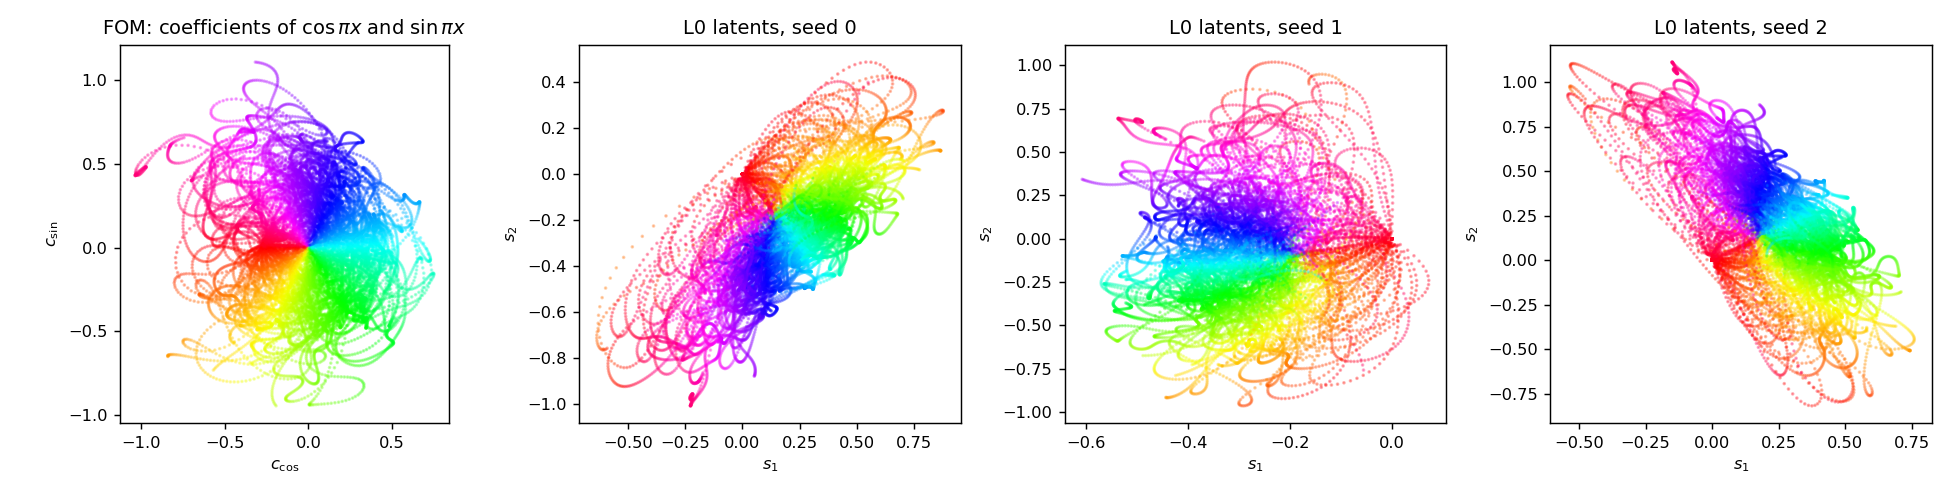
\includegraphics[width=0.90\textwidth,height=0.215\textheight,keepaspectratio]{fig9_A_latents.png}
  \caption{Curved latent coordinates learned by $\mathrm{L0}$ in Case~A ($d_s = 2$). \textbf{Left:} true Fourier coefficients $(c_{\cos}, c_{\sin})$ of the centred test fields, coloured by phase angle. \textbf{Right:} learned latent trajectories $(s_1(t), s_2(t))$ of $\mathrm{L0}$ across the three random seeds $\{0,1,2\}$ for the exact same test states and colour map. The circular modal phase space is preserved topologically but sheared and radially compressed by a cubic distortion ($R^2_{\mathrm{lin}} = 0.55$, cubic $R^2 = 0.98$).}
  \label{fig:rq2_fig9}
\end{figure}

\subsection{Case B Results: Navier--Stokes Cavity Flow, Quiescent Corners, and Preconditioning}

Table~\ref{tab:rq2_caseB} reports the \texttt{RQ2} results for the 2D lid-driven cavity flow at the 200 Adam + 500 BFGS budget.

\begin{table}[!htbp]
\centering
\caption{Case B (\texttt{2D-Stokes}) results in \texttt{RQ2} (200 Adam + 500 BFGS epochs). \textbf{Top:} validation-selected best configuration of each procedure and goal-oriented physical metrics (direction error, relative vorticity error, and time-extrapolation ratio $\varepsilon_{[20,40]}/\varepsilon_{[0,20]}$). \textbf{Bottom:} $K$-sweep at $d_s = 10$.}
\label{tab:rq2_caseB}
\footnotesize\resizebox{\textwidth}{!}{%

\begin{tabular}{@{}lrrrlrrrrrr@{}}
\toprule
\textbf{Procedure} & $d_s$ & $K$ & $P_{\mathrm{rec}}$ & \textbf{Test NRMSE $[\min, \max]$} & \textbf{Ratio L0} & \textbf{Dir.\ Err.} & \textbf{Vort.\ Err.} & \textbf{Extrap.} & \textbf{Train [s]} & \textbf{Infer [ms]} \\
\midrule
$\mathrm{L0}$ (R2) & $10$ & -- & $2186$ & $1.97\cdot 10^{-2}$ $[1.89, 2.25]\cdot 10^{-2}$ & $1.00$ & $0.051$ & $0.887$ & $0.974$ & $240.0$ & $931.9$ \\
$\mathrm{L1}$-R1 & $1$ & $1$ & $0$ & $3.66\cdot 10^{-2}$ $[2.93, 6.02]\cdot 10^{-2}$ & $1.86$ & $0.323$ & $0.765$ & $0.980$ & $0.0$ & $12.3$ \\
$\mathrm{L1}$-R2 & $5$ & $5$ & $0$ & $8.69\cdot 10^{-3}$ $[7.92, 9.16]\cdot 10^{-3}$ & $0.44$ & $0.048$ & $0.241$ & $0.968$ & $38.4$ & $8.0$ \\
$\mathrm{L2}$-R1 & $10$ & $5$ & $60$ & $1.53\cdot 10^{-2}$ $[1.39, 1.77]\cdot 10^{-2}$ & $0.77$ & $0.098$ & $0.411$ & $1.007$ & $28.0$ & $8.4$ \\
$\mathrm{L2}$-R2 & $5$ & $17$ & $119$ & $8.06\cdot 10^{-3}$ $[7.98, 8.91]\cdot 10^{-3}$ & $0.41$ & $0.028$ & $0.232$ & $1.065$ & $46.0$ & $10.2$ \\
$\mathbf{L3}$\textbf{-R1} & $\mathbf{10}$ & $\mathbf{10}$ & $\mathbf{2134}$ & $\mathbf{4.43\cdot 10^{-3}}$ $[4.21, 4.51]\cdot 10^{-3}$ & $\mathbf{0.22}$ & $\mathbf{0.026}$ & $\mathbf{0.110}$ & $\mathbf{0.774}$ & $\mathbf{92.0}$ & $\mathbf{12.7}$ \\
$\mathbf{L3}$\textbf{-R2} & $\mathbf{10}$ & $\mathbf{10}$ & $\mathbf{2134}$ & $\mathbf{4.52\cdot 10^{-3}}$ $[4.27, 4.72]\cdot 10^{-3}$ & $\mathbf{0.23}$ & $\mathbf{0.025}$ & $\mathbf{0.123}$ & $\mathbf{0.747}$ & $\mathbf{110.2}$ & $\mathbf{10.4}$ \\
\bottomrule
\end{tabular}
}

\vspace{0.6em}\resizebox{\textwidth}{!}{%

\begin{tabular}{@{}lccccc@{}}
\toprule
\textbf{K-Sweep at $d_s = 10$} & $K = 3$ & $K = 5$ & $K = 9$ & $K = 10$ & $K = 17$ \\
\midrule
$\mathrm{L2}$-R2 test NRMSE ($\eta = \varepsilon_{\mathrm{total}}/\varepsilon_{\mathrm{proj}}$) & $1.23\cdot 10^{-2}$ ($2.8$) & $9.75\cdot 10^{-3}$ ($4.0$) & $1.00\cdot 10^{-2}$ ($10.2$) & $8.07\cdot 10^{-3}$ ($9.8$) & $8.99\cdot 10^{-3}$ ($26.0$) \\
$\mathrm{L2}$-R1 test NRMSE (frozen $\mathrm{L0}$ latents) & $1.71\cdot 10^{-2}$ & $1.53\cdot 10^{-2}$ & $1.69\cdot 10^{-2}$ & $1.69\cdot 10^{-2}$ & $1.66\cdot 10^{-2}$ \\
$\mathrm{L3}$-R2 test NRMSE ($\eta = \varepsilon_{\mathrm{total}}/\varepsilon_{\mathrm{proj}}$) & $1.15\cdot 10^{-2}$ ($2.6$) & $1.07\cdot 10^{-2}$ ($4.4$) & $5.16\cdot 10^{-3}$ ($5.2$) & $4.52\cdot 10^{-3}$ ($5.5$) & $4.74\cdot 10^{-3}$ ($13.7$) \\
$\mathrm{L3}$-R1 test NRMSE (frozen $\mathrm{L0}$ latents) & $1.00\cdot 10^{-2}$ & $6.38\cdot 10^{-3}$ & $5.05\cdot 10^{-3}$ & $4.43\cdot 10^{-3}$ & $4.75\cdot 10^{-3}$ \\
Matched hidden width $w_g$ of $\mathrm{L3}$ & $39$ & $38$ & $36$ & $36$ & $33$ \\
\bottomrule
\end{tabular}
}
\end{table}

At the 500-BFGS-epoch budget of \texttt{RQ2}, replacing the pointwise MLP $\mathrm{L0}$ ($1.97\cdot 10^{-2}$) with vector POD modes yields dramatic gains across all modal variants: even the parameter-free identity $\mathrm{L1}$-R2 reaches $8.69\cdot 10^{-3}$ ($2.3\times$ lower error than $\mathrm{L0}$), the affine map $\mathrm{L2}$-R2 reaches $8.06\cdot 10^{-3}$ ($2.4\times$ lower error with $18\times$ fewer decoder parameters), and the nonlinear coefficient map $\mathrm{L3}$ reaches $4.52\cdot 10^{-3}$ in R2 and $4.43\cdot 10^{-3}$ in R1 ($4.4\times$ lower NRMSE and $8\times$ lower vorticity error than $\mathrm{L0}$, while accelerating test-set decoder evaluation by $90\times$, from $932$~ms to $10.4$~ms). However, notice that for $K \ge 10$, the efficiency ratios $\eta = \varepsilon_{\mathrm{total}}/\varepsilon_{\mathrm{proj}}(K)$ are large ($9.8$--$26.0$ for $\mathrm{L2}$, $5.5$--$13.7$ for $\mathrm{L3}$): the POD basis is already capable of $\NRMSE \le 8\cdot 10^{-4}$, so both the small canonical $7\text{--}7$ dynamics network and the 500-iteration BFGS cap limit accuracy---a diagnosis that \texttt{RQ2-bis} confirms and resolves in Section~\ref{sec:rq2bis}.

\begin{figure}[!htbp]
  \centering
  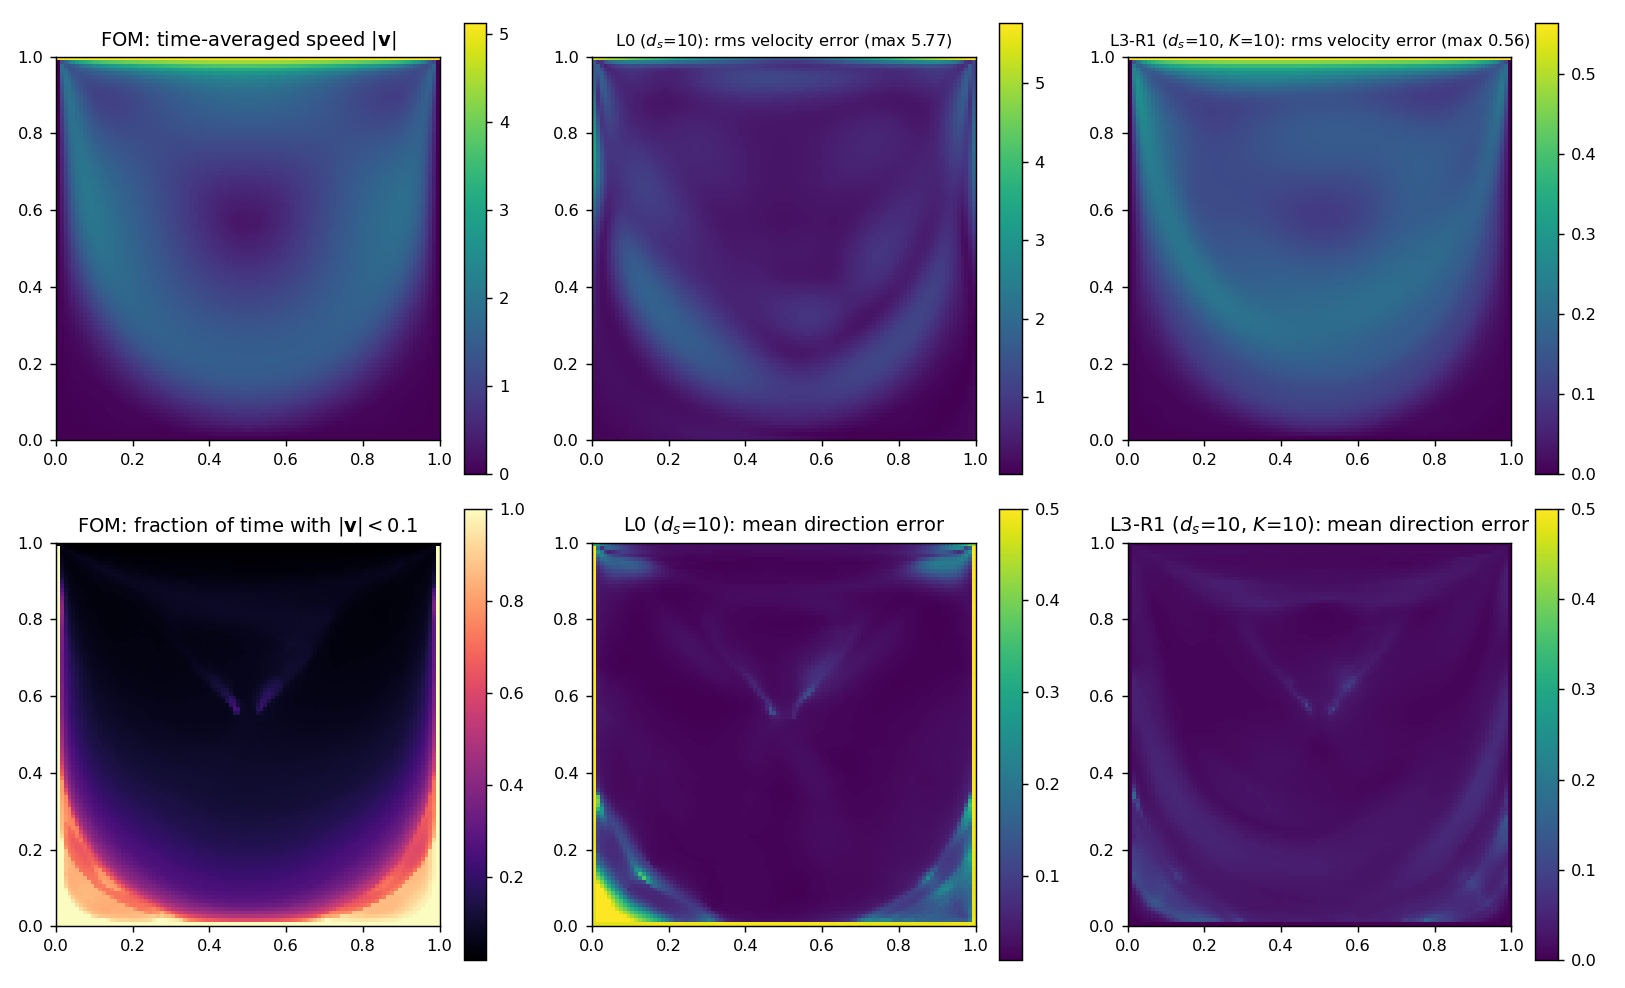
\includegraphics[width=0.90\textwidth,height=0.215\textheight,keepaspectratio]{fig8_B_maps.png}
  \caption{Spatial anatomy of velocity and direction errors in Case~B ($d_s = 10$, test set). \textbf{Top row:} time-averaged speed $\norm{\mathbf{v}}_2$ of the true FOM flow (left), and pointwise rms velocity error of $\mathrm{L0}$ (centre, max $0.68$) and $\mathrm{L3}$-R1 (right, max $0.17$). \textbf{Bottom row:} fraction of time steps where the true speed is below $0.1$ (left), and time-averaged direction error $\norm{\mathbf{d}(\hat{\mathbf{v}}) - \mathbf{d}(\mathbf{v})}^2$ of $\mathrm{L0}$ (centre) and $\mathrm{L3}$-R1 (right).}
  \label{fig:rq2_fig8}
\end{figure}

Figure~\ref{fig:rq2_fig8} resolves Hypothesis~H3 regarding where the direction error~\eqref{eq:caseB_loss} originates. Because the unit-vector map $\mathbf{d}(\mathbf{v}) = \mathbf{v}/(10^{-4} + \norm{\mathbf{v}})$ has Jacobian scaling as $1/\norm{\mathbf{v}}$, it is ill-conditioned wherever the flow speed $\norm{\mathbf{v}}$ is small: $22.0\%$ of space-time test points have speed $\norm{\mathbf{v}} < 0.1$ (compared with lid speeds of order $10$), yet they account for \textbf{$77.0\%$ of the total direction error in $\mathrm{L0}$ and $89.5\%$ in $\mathrm{L3}$-R1} (points with $\norm{\mathbf{v}} < 0.01$ alone carry $54.4\%$ and $47.3\%$). Consequently, the direction error is concentrated not at the two upper singular lid corners (which carry only $6.9\%$ of the direction error in $\mathrm{L0}$ and $1.4\%$ in $\mathrm{L3}$-R1), but rather in the quiescent bottom strip of the cavity ($30.6\%$ and $16.5\%$), along the stationary walls, at the zero-velocity centre of the primary vortex, and along the separatrix between the primary and secondary corner vortices.

\subsection{Case C Results: Travelling Fronts, the Kolmogorov Barrier, and the Threshold at \texorpdfstring{$d_s = 3$}{ds = 3}}

Table~\ref{tab:rq2_caseC} and Figure~\ref{fig:rq2_fig7} present the \texttt{RQ2} results for the 1D Aliev--Panfilov electrophysiology benchmark.

\begin{table}[!htbp]
\centering
\caption{Case C (\texttt{AP1D}) results in \texttt{RQ2} (200 Adam + 500 BFGS epochs). \textbf{Top:} validation-selected best configuration of each procedure and front activation-time MAE (ms). \textbf{Bottom:} $K$-sweep at $d_s = 12$ and $d_s$-sweep of $\mathrm{L0}$ vs.\ $\mathrm{L1}$.}
\label{tab:rq2_caseC}
\footnotesize\resizebox{\textwidth}{!}{%

\begin{tabular}{@{}lrrrlrrlrrr@{}}
\toprule
\textbf{Procedure} & $d_s$ & $K$ & $P_{\mathrm{rec}}$ & \textbf{Test NRMSE $[\min, \max]$} & $\varepsilon_{\mathrm{total}}$ & \textbf{Ratio L0} & \textbf{Sep.} & \textbf{Act.\ MAE [ms]} & \textbf{Train [s]} & \textbf{Infer [ms]} \\
\midrule
$\mathbf{L0}$ \textbf{(R2)} & $\mathbf{5}$ & -- & $\mathbf{1361}$ & $\mathbf{1.76\cdot 10^{-2}}$ $[1.58, 3.27]\cdot 10^{-2}$ & $\mathbf{0.051}$ & $\mathbf{1.00}$ & -- & $\mathbf{1.00}$ $[0.92, 1.54]$ & $\mathbf{133.7}$ & $\mathbf{366.8}$ \\
$\mathrm{L1}$-R1 & $1$ & $1$ & $0$ & $3.15\cdot 10^{-1}$ $[3.02, 3.20]\cdot 10^{-1}$ & $0.904$ & $17.86$ & yes & $319.1$ & $0.0$ & $4.0$ \\
$\mathrm{L1}$-R2 & $12$ & $12$ & $0$ & $1.22\cdot 10^{-1}$ $[1.20, 1.32]\cdot 10^{-1}$ & $0.350$ & $6.92$ & yes & $8.35$ $[8.34, 8.42]$ & $22.5$ & $1.9$ \\
$\mathrm{L2}$-R1 & $12$ & $33$ & $429$ & $1.94\cdot 10^{-1}$ $[1.76, 2.12]\cdot 10^{-1}$ & $0.556$ & $10.99$ & yes & $26.56$ $[19.6, 45.4]$ & $16.0$ & $6.1$ \\
$\mathrm{L2}$-R2 & $12$ & $33$ & $429$ & $1.01\cdot 10^{-1}$ $[1.00, 1.03]\cdot 10^{-1}$ & $0.290$ & $5.73$ & yes & $5.10$ $[4.89, 5.38]$ & $27.5$ & $3.0$ \\
$\mathrm{L3}$-R1 & $12$ & $17$ & $1417$ & $6.62\cdot 10^{-2}$ $[6.36, 6.86]\cdot 10^{-2}$ & $0.190$ & $3.75$ & yes & $2.78$ $[2.70, 2.89]$ & $34.0$ & $14.2$ \\
$\mathrm{L3}$-R2 & $12$ & $17$ & $1417$ & $6.93\cdot 10^{-2}$ $[6.69, 7.02]\cdot 10^{-2}$ & $0.199$ & $3.93$ & yes & $2.80$ $[2.70, 2.97]$ & $51.7$ & $5.0$ \\
\bottomrule
\end{tabular}
}

\vspace{0.6em}\resizebox{\textwidth}{!}{%

\begin{tabular}{@{}lcccc@{\hspace{2em}}lccccc@{}}
\toprule
\textbf{K-Sweep ($d_s=12$)} & $K=5$ & $K=12$ & $K=17$ & $K=33$ & \textbf{$d_s$-Sweep} & $d_s=1$ & $d_s=2$ & $d_s=3$ & $d_s=5$ & $d_s=12$ \\
\midrule
$\mathrm{L2}$-R2 NRMSE & $0.159$ & $0.103$ & $0.102$ & $0.101$ & $\mathrm{L0}$ (R2) & $0.134$ & $0.120$ & $\mathbf{0.0176}$ & $\mathbf{0.0176}$ & $0.0221$ \\
$\mathrm{L2}$-R2 $\eta = \varepsilon/\varepsilon_{\mathrm{proj}}$ & $1.06$ & $1.38$ & $1.85$ & $4.11$ & $\mathrm{L1}$-R2 & $0.281$ & $0.252$ & $0.236$ & $0.166$ & $0.122$ \\
$\mathrm{L3}$-R2 NRMSE & $0.150$ & $0.0809$ & $0.0693$ & $0.0693$ & $\mathrm{L1}$-R1 & $0.315$ & $0.327$ & $0.385$ & $0.373$ & $0.365$ \\
$\mathrm{L3}$-R2 $\eta = \varepsilon/\varepsilon_{\mathrm{proj}}$ & $1.00$ & $1.08$ & $1.26$ & $2.82$ & Seed align $R^2$ ($\mathrm{L0}$) & $0.015$ & $0.641$ & $\mathbf{0.970}$ & $\mathbf{0.985}$ & $\mathbf{0.991}$ \\
\bottomrule
\end{tabular}
}
\end{table}

Case~C provides an unequivocal demonstration of why the non-separable pointwise MLP reconstructor $\mathrm{L0}$ was invented:
\begin{enumerate}[leftmargin=2em]
  \item \textbf{Complete failure of fixed-basis decoders ($\mathrm{L1}$--$\mathrm{L3}$) against moving fronts:} No fixed-basis reconstructor comes closer to $\mathrm{L0}$ ($1.76\cdot 10^{-2}$, relative error $\varepsilon_{\mathrm{total}} = 5.0\%$, activation-time MAE $1.00$~ms) than a factor of \textbf{$3.75\times$} ($\mathrm{L3}$-R1 at $6.62\cdot 10^{-2}$) or \textbf{$5.73\times$} ($\mathrm{L2}$-R2 at $1.01\cdot 10^{-1}$). As shown in Table~\ref{tab:rq2_caseC} (bottom left), $\mathrm{L2}$-R2 hugs the Legendre projection floor at $K=5$ ($\eta = 1.06$), slows down at $K=12$ ($\eta = 1.38$), and completely stagnates at $0.101$--$0.103$ for $K \in \{12, 17, 33\}$ ($\eta$ rising to $4.11$) because of the 12-dimensional rank bound $\varepsilon_{\mathrm{rank}}(12) = 0.1447$. Even when $\mathrm{L3}$ uses a parameter-matched nonlinear MLP $g_\theta(\mathbf{s})$ to curve the 12-dimensional manifold inside $V_K$, it is pinned directly against the Legendre projection floor up to $K=17$ ($\eta = 1.00$ at $K=5$, $1.08$ at $K=12$, $1.26$ at $K=17$) and stalls at $6.93\cdot 10^{-2}$ at $K=33$ as its matched hidden width shrinks from $30$ to $21$.
  \item \textbf{Sharp phase transition of $\mathrm{L0}$ at the intrinsic dimension $d_s = 3$:} As $d_s$ increases from $1$ to $2$ to $3$, the test NRMSE of $\mathrm{L0}$ drops abruptly by \textbf{$7\times$}, from $0.134$ ($d_s=1$) and $0.120$ ($d_s=2$) to \textbf{$1.76\cdot 10^{-2}$} at $d_s=3$ ($\varepsilon_{\mathrm{total}} = 0.050$, $8.5\times$ below the 3-mode POD rank floor $0.4261$!), and remains on a plateau for $d_s = 5$ ($1.76\cdot 10^{-2}$) and $d_s = 12$ ($2.21\cdot 10^{-2}$). Simultaneously, the cross-seed affine alignment $R^2$ between the latent trajectories of different seeds jumps from $0.015$ ($d_s=1$) and $0.641$ ($d_s=2$) to \textbf{$0.970$, $0.985$, and $0.991$} for $d_s = 3, 5, 12$. Three latent variables suffice to parameterise the positions and recovery states of the two colliding depolarisation waves, and $\NNrec(\mathbf{s},x)$ translates the steep wave profiles directly in $x$ as a function of $\mathbf{s}(t)$ without Gibbs oscillations (Figure~\ref{fig:rq2_fig7}).
\end{enumerate}

\begin{figure}[!htbp]
  \centering
  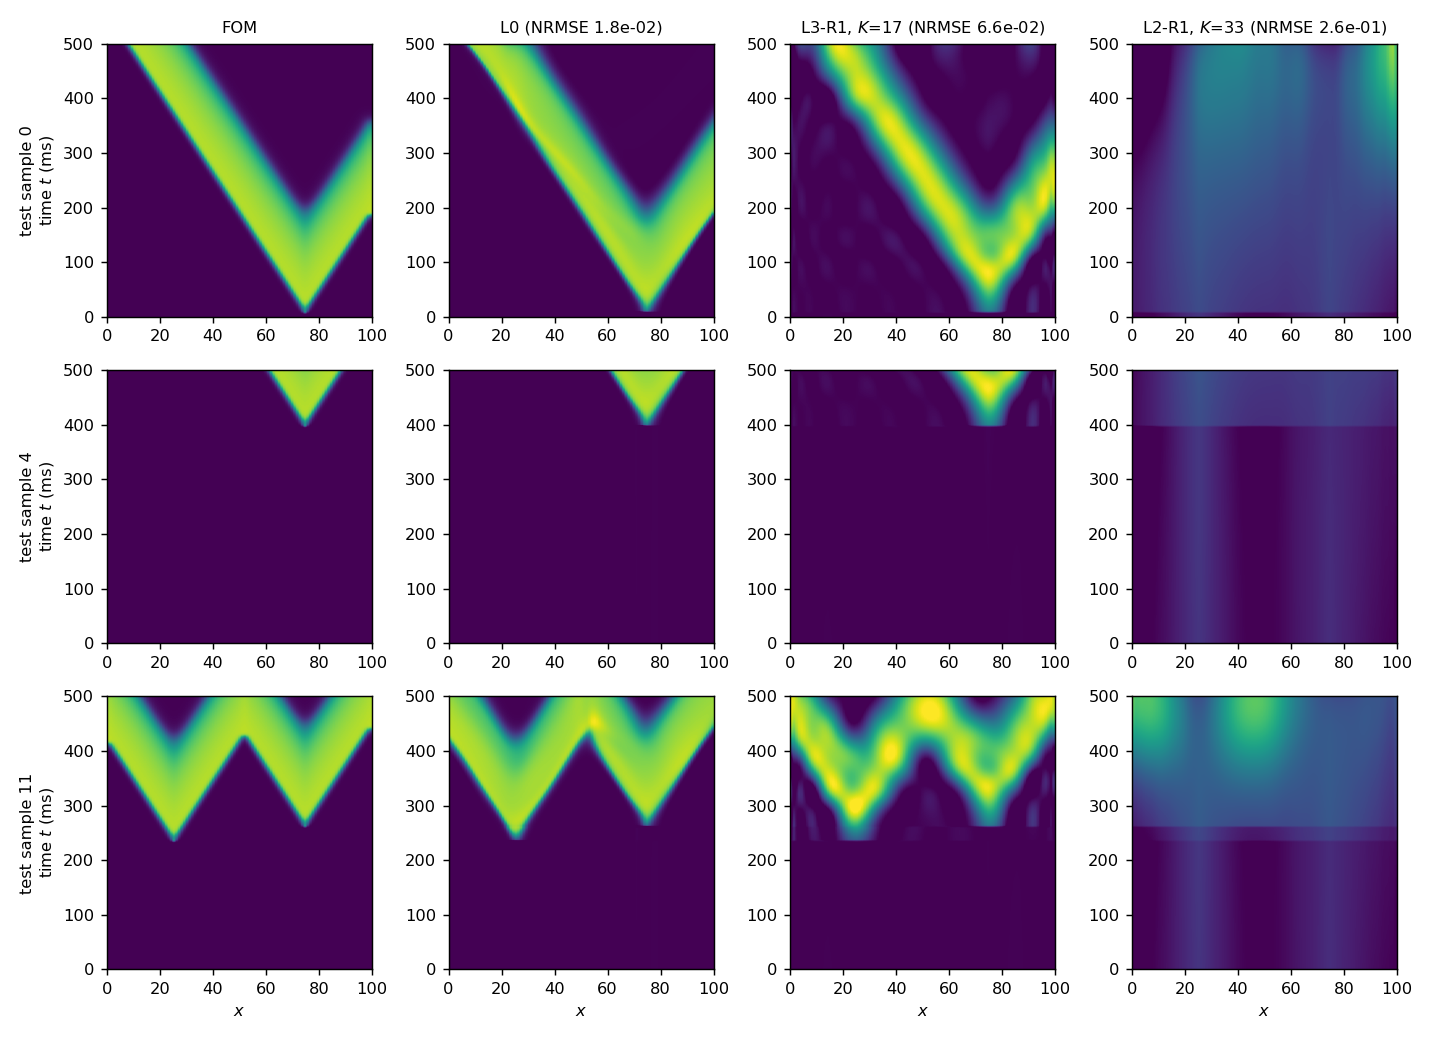
\includegraphics[width=0.90\textwidth,height=0.215\textheight,keepaspectratio]{fig7_C_decoders.png}
  \caption{Space-time transmembrane potential $y(x,t)$ across three test trajectories of Case~C (rows), decoded from the \emph{exact same frozen $\mathrm{L0}$ latent trajectory} ($d_s = 5$, Regime~R1). \textbf{Columns:} FOM ground truth; original implicit MLP $\mathrm{L0}$ ($\NRMSE = 1.76\cdot 10^{-2}$); nonlinear modal decoder $\mathrm{L3}$ ($K=17$, $\NRMSE = 6.62\cdot 10^{-2}$); and affine modal decoder $\mathrm{L2}$ ($K=33$, $\NRMSE = 1.94\cdot 10^{-1}$). The frozen $\mathrm{L0}$ latents trigger the wave onset at the exact right millisecond in every decoder, but fixed polynomial bases ($\mathrm{L2}, \mathrm{L3}$) smear the steep depolarisation fronts and introduce severe Gibbs ringing.}
  \label{fig:rq2_fig7}
\end{figure}

\subsection{Cross-Case Synthesis: Error vs.\ \texorpdfstring{$K$}{K}, Error vs.\ \texorpdfstring{$d_s$}{ds}, and Parameter Pareto Fronts}

Figures~\ref{fig:rq2_fig2}, \ref{fig:rq2_fig3}, and~\ref{fig:rq2_fig5} synthesise the 816 runs of \texttt{RQ2} across all three PDE benchmarks.

\begin{figure}[!htbp]
  \centering
  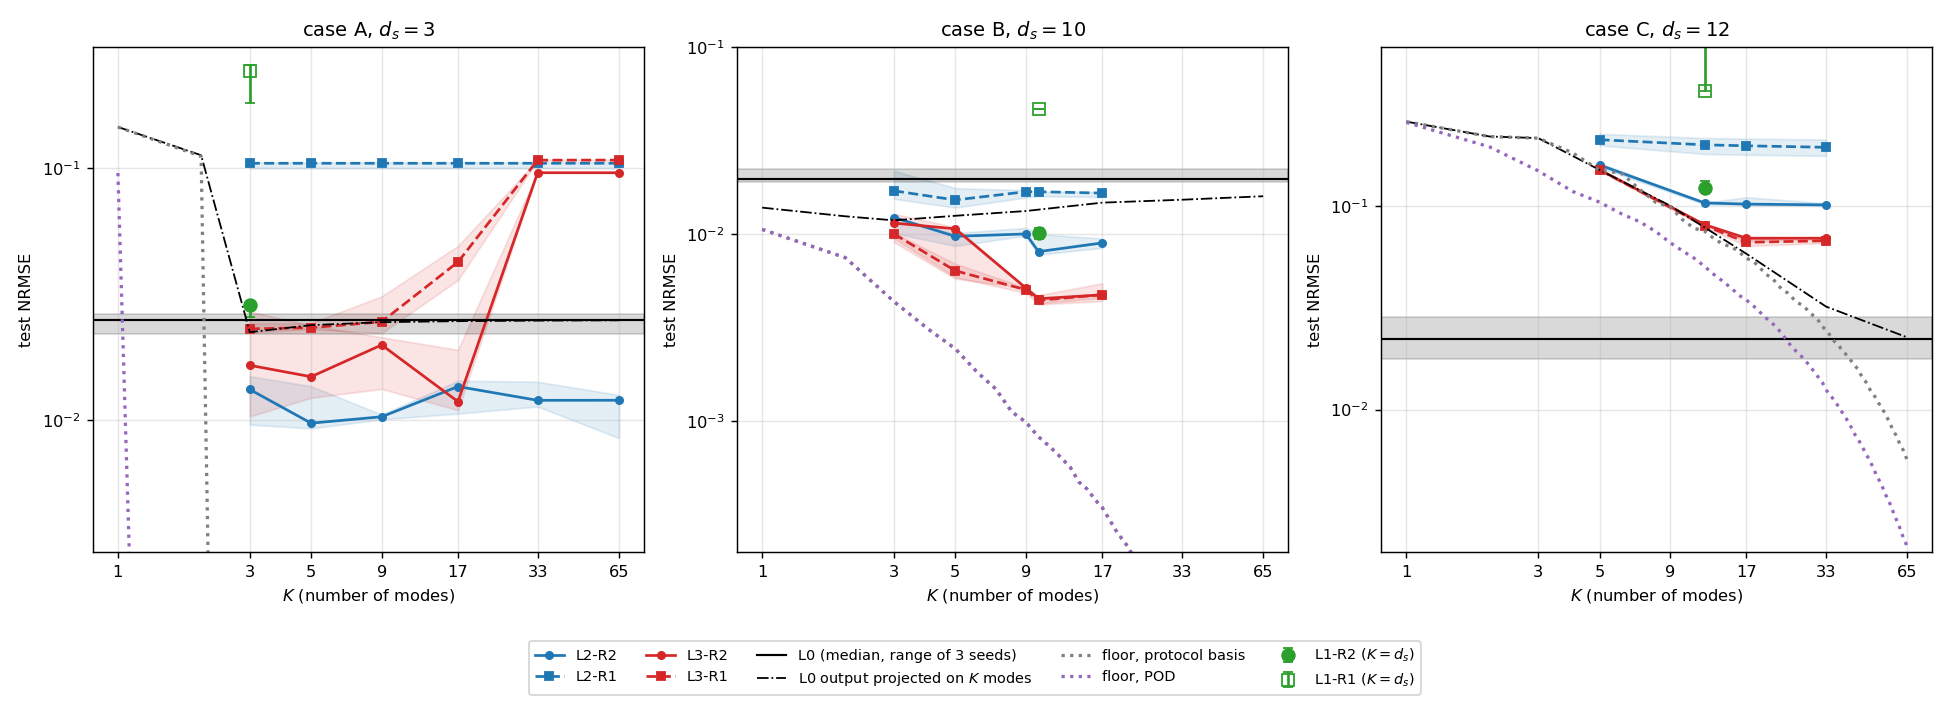
\includegraphics[width=0.90\textwidth,height=0.215\textheight,keepaspectratio]{fig2_error_vs_K.png}
  \caption{The core \texttt{RQ2} comparison: test NRMSE (median and min--max band over 3 seeds) against the number of basis modes $K$ at reference latent dimensions $d_s = 3$ (Case~A), $d_s = 10$ (Case~B), and $d_s = 12$ (Case~C). Solid lines denote end-to-end training ($\mathrm{R2}$) and dashed lines denote frozen-latent fitting ($\mathrm{R1}$) for $\mathrm{L2}$ (blue) and $\mathrm{L3}$ (red), alongside $\mathrm{L1}$ at $K=d_s$ (green), the $\mathrm{L0}$ seed band (grey shaded), the $\mathrm{L0}$ output orthogonally projected onto $K$ modes (black dash-dotted), and the projection floors $\varepsilon_{\mathrm{proj}}(K)$ (dotted).}
  \label{fig:rq2_fig2}
\end{figure}

\begin{figure}[!htbp]
  \centering
  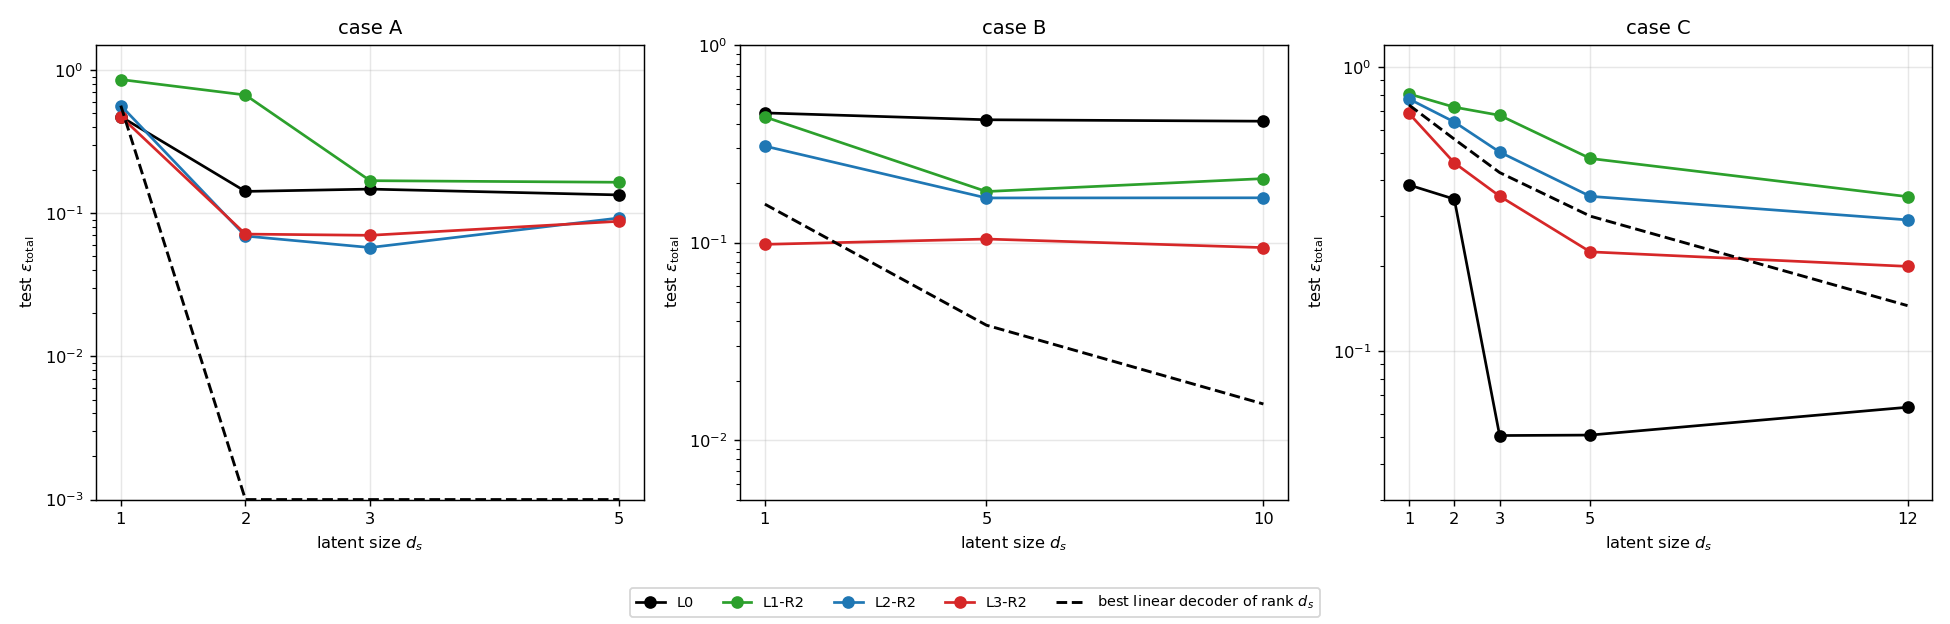
\includegraphics[width=0.90\textwidth,height=0.215\textheight,keepaspectratio]{fig3_rank_bound.png}
  \caption{Verification of the Reconstructor Rank Bound (Proposition~\ref{prop:rec_rank_bound}): relative test error $\varepsilon_{\mathrm{total}}$ against latent size $d_s$ for $\mathrm{L0}$, $\mathrm{L1}$-R2, $\mathrm{L2}$-R2, and $\mathrm{L3}$-R2 (with $K$ selected on validation), compared against the linear rank floor $\varepsilon_{\mathrm{rank}}(r)$ of the leading $r$ POD modes (black dashed; $r = d_s$ in Cases~A and~C, $r = d_s + 1$ in Case~B).}
  \label{fig:rq2_fig3}
\end{figure}

\begin{figure}[!htbp]
  \centering
  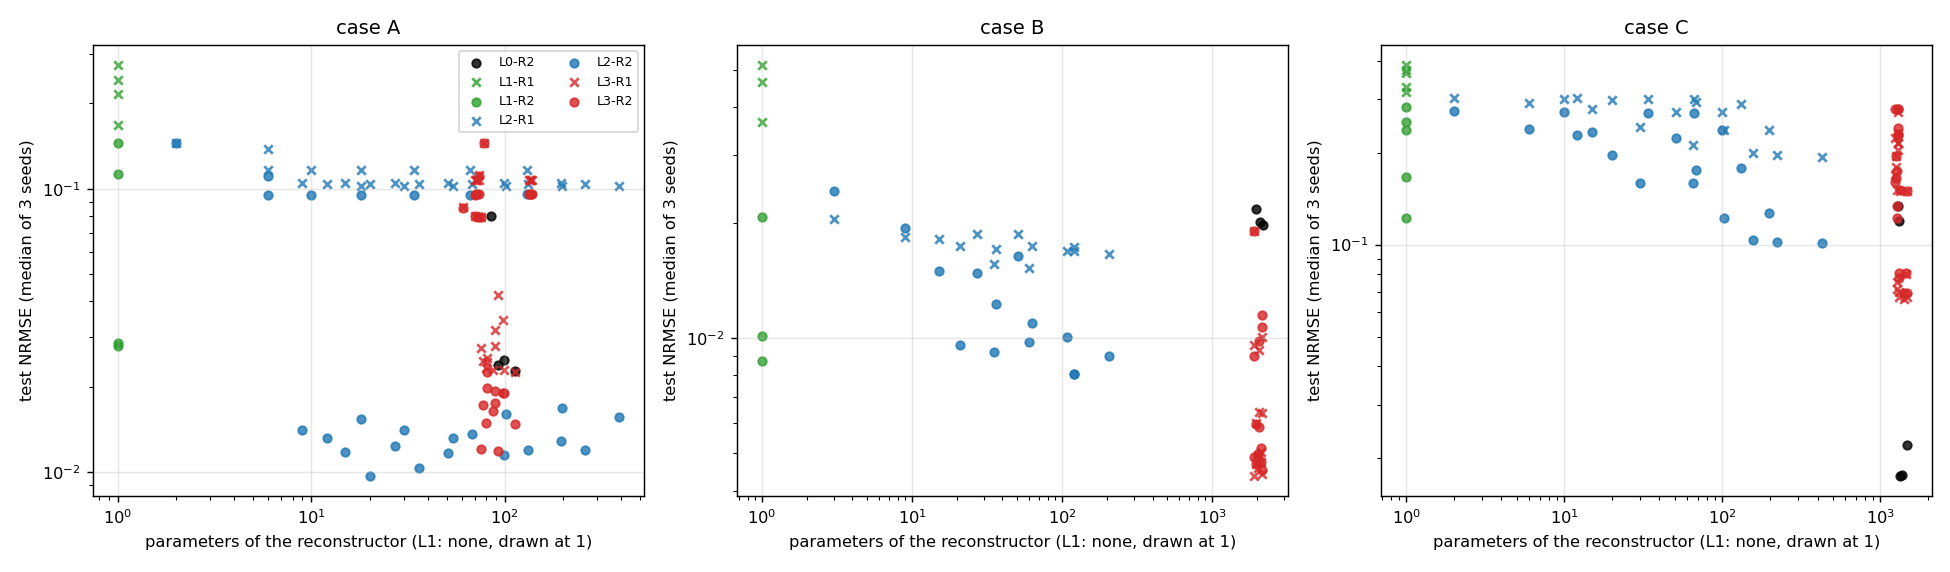
\includegraphics[width=0.90\textwidth,height=0.215\textheight,keepaspectratio]{fig5_pareto.png}
  \caption{Test NRMSE (median of 3 seeds) against reconstructor parameter count $P_{\mathrm{rec}}$ across all configurations of the \texttt{RQ2} sweeps in Cases~A, B, and~C (circles: end-to-end Regime~R2; crosses: frozen-latent Regime~R1; $\mathrm{L1}$ has $P_{\mathrm{rec}}=0$ and is plotted at $1$).}
  \label{fig:rq2_fig5}
\end{figure}

Figure~\ref{fig:rq2_fig3} confirms Proposition~\ref{prop:rec_rank_bound} across every single configuration of the study: the affine modal decoder $\mathrm{L2}$-R2 (blue curve) \textbf{never crosses below the black dashed rank floor $\varepsilon_{\mathrm{rank}}(r)$} (sitting directly on it at $d_s=1$ in Case~A, $0.566$ vs.\ $0.565$, and remaining above it everywhere in Cases~B and~C). By contrast, the nonlinear decoders breaks through the linear rank floor whenever $d_s$ is small: $\mathrm{L3}$-R2 goes below $\varepsilon_{\mathrm{rank}}(r)$ at $d_s=1$ in Case~A ($0.474$ vs.\ $0.565$), at $d_s=1$ in Case~B ($0.098$ vs.\ $0.156$), and at every $d_s \le 5$ in Case~C ($0.352$ vs.\ $0.426$ at $d_s=3$; $0.224$ vs.\ $0.299$ at $d_s=5$), while $\mathrm{L0}$ breaks the rank floor by a factor of $8.5\times$ in Case~C at $d_s=3$ ($0.050$ vs.\ $0.426$).

\subsection{Spectral Probing of the Trained \texorpdfstring{$\mathrm{L0}$}{L0} Decoder, Linear Invariants, and the Initial-State Handicap}
\label{sec:rq2_spectral_probing}

To understand how the trained implicit MLP $\NNrec(\mathbf{z},\mathbf{x})$ behaves internally on the states it visits, we project its test-set output $\hat{y}_{\mathrm{L0}}(\cdot,t) - \bar{y}$ onto the orthonormal basis $\{\varphi_k\}$ to extract its modal coefficients $\hat{c}_k^{\mathrm{L0}}(t) = \ip{\hat{y}_{\mathrm{L0}}(\cdot,t) - \bar{y}}{\varphi_k}$, and compute two diagnostic quantities defined in the protocol:
\begin{enumerate}[leftmargin=2em]
  \item The \textbf{linearizability index} $R^2_{\mathrm{lin}}(K)$, defined as the coefficient of determination of the best affine least-squares fit $\hat{\mathbf{c}}_{1:K}^{\mathrm{L0}}(t) \approx W\mathbf{z}(t) + \mathbf{b}$ over all test trajectories and time steps:
  \begin{equation}
    R^2_{\mathrm{lin}}(K) = 1 - \frac{\sum_{s,i} \norm{\hat{\mathbf{c}}_{1:K}^{\mathrm{L0}}(t_i) - \big(W\mathbf{z}^{(s)}(t_i) + \mathbf{b}\big)}_2^2}{\sum_{s,i} \norm{\hat{\mathbf{c}}_{1:K}^{\mathrm{L0}}(t_i) - \overline{\hat{\mathbf{c}}}_{1:K}^{\mathrm{L0}}}_2^2}.
    \label{eq:R2_lin}
  \end{equation}
  \item The \textbf{effective spectral width} $K_{99}$, defined at each test snapshot as the smallest mode count $K \le 65$ holding at least $99\%$ of the modal energy $\sum_{k=1}^{65} |\hat{c}_k(t)|^2$.
\end{enumerate}

\begin{figure}[!htbp]
  \centering
  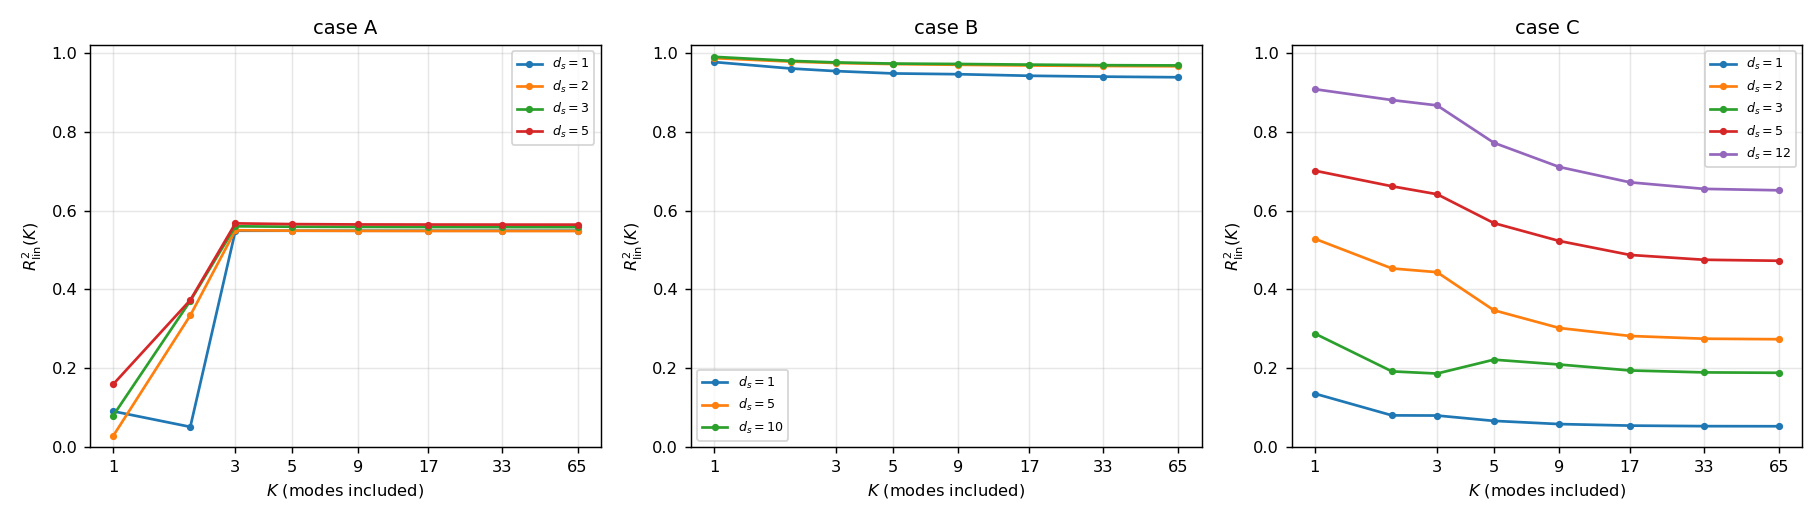
\includegraphics[width=0.90\textwidth,height=0.215\textheight,keepaspectratio]{fig4_L0_linearity.png}
  \caption{Linearizability index $R^2_{\mathrm{lin}}(K)$ of the trained $\mathrm{L0}$ reconstructor~\eqref{eq:R2_lin} against the number of included modes $K$ across latent dimensions $d_s$ (median of 3 seeds) for Case~A (left), Case~B (centre), and Case~C (right).}
  \label{fig:rq2_fig4}
\end{figure}

\begin{figure}[!htbp]
  \centering
  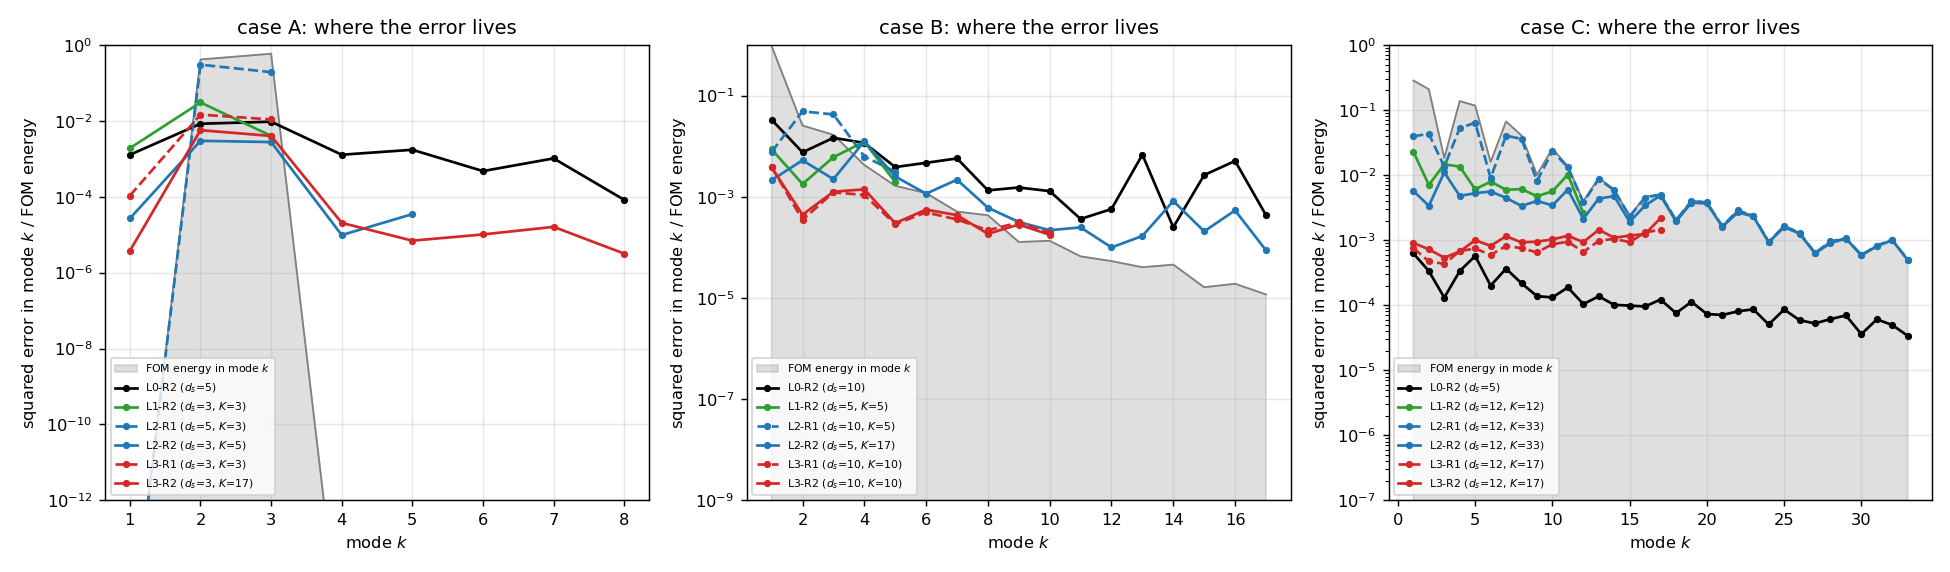
\includegraphics[width=0.90\textwidth,height=0.215\textheight,keepaspectratio]{fig6_modes.png}
  \caption{Per-mode coefficient error spectra $\norm{\hat{c}_k - c_k}_2$ (and true modal energy $\norm{c_k}_2$, black) across mode index $k$ at the reference latent size of each case in \texttt{RQ2}. Notice the spurious high-frequency spectral tail of $\mathrm{L0}$ for $k \ge 4$ in Case~A and $k \ge 10$ in Case~B.}
  \label{fig:rq2_fig6}
\end{figure}

Figures~\ref{fig:rq2_fig4} and~\ref{fig:rq2_fig6} reveal three deep structural properties of implicit MLP decoders versus modal expansions:
\begin{itemize}[leftmargin=2em]
  \item \textbf{Spurious high-wavenumber tails in $\mathrm{L0}$ and denoising via modal projection:} In Case~B, the true velocity field has a narrow spectral width of $K_{99} = 4$ POD modes (interquartile range $[2,6]$), and $\mathrm{L0}$ is almost perfectly affine in its inputs on the visited states ($R^2_{\mathrm{lin}}(K) \in [0.94, 0.99]$, Figure~\ref{fig:rq2_fig4} centre). Yet $\mathrm{L0}$'s output exhibits a massive spurious high-frequency tail with \textbf{$K_{99} = 42$ modes} (Figure~\ref{fig:rq2_fig6} centre)! Because spatial differentiation multiplies mode $k$ by its characteristic wavenumber, this spurious tail inflates $\mathrm{L0}$'s relative vorticity error in \texttt{RQ2} to $0.887$. Simply projecting $\mathrm{L0}$'s predicted velocity field onto the first $K=3$ POD modes (dash-dotted black curve in Figure~\ref{fig:rq2_fig2} centre) \textbf{reduces $\mathrm{L0}$'s test NRMSE by $40\%$} (from $1.97\cdot 10^{-2}$ to $1.19\cdot 10^{-2}$) and cuts its vorticity error from $0.887$ to $0.268$! Similarly, projecting $\mathrm{L0}$ onto $K=3$ Fourier modes in Case~A lowers its NRMSE by $10\%$ ($2.49\cdot 10^{-2} \to 2.23\cdot 10^{-2}$). Conversely, in Case~C both the FOM and $\mathrm{L0}$ have $K_{99} = 25$ modes, and projecting $\mathrm{L0}$ onto $K \le 33$ modes destroys the sharp front profile ($2.21\cdot 10^{-2} \to 3.20\cdot 10^{-2}$ at $K=33$ and $5.82\cdot 10^{-2}$ at $K=17$).
  \item \textbf{Inheritance of linear physical invariants (discrete incompressibility):} Because every vector POD mode $\boldsymbol{\varphi}_k(\mathbf{x})$ in Case~B is a linear combination of divergence-free FOM velocity snapshots, any modal expansion $\hat{\mathbf{v}} = \bar{\mathbf{v}} + \sum_{k=1}^K c_k(t)\boldsymbol{\varphi}_k(\mathbf{x})$ automatically inherits the discrete divergence level of the FOM grid: measuring $\norm{\nabla\cdot\mathbf{v}}_2 / \norm{\nabla\mathbf{v}}_2$ by central differences on the $100\times 100$ grid yields \textbf{$0.0696$ for the FOM and $0.0696$ ($[0.0693, 0.0699]$) for $\mathrm{L3}$-R1}, whereas the unconstrained pointwise MLP $\mathrm{L0}$ gives $0.270$ ($[0.210, 0.331]$, nearly $4\times$ higher divergence in \texttt{RQ2}, and still $1.9\times$ higher even after $10{,}000$ BFGS iterations in \texttt{RQ2-bis}).
  \item \textbf{The initial-state handicap of $\mathrm{L1}$:} Because all modal variants add the non-zero time-averaged training field $\bar{y}(\mathbf{x})$ ($\mathrm{rms}(\bar{y})/\mathrm{rms}(y) = 0.520, 0.175, 0.481$ in Cases~A, B, C) while the latent ODE starts at $\mathbf{s}(0) = \mathbf{0}$, the parameter-free identity decoder $\mathrm{L1}$ ($\hat{y}(\cdot,0) = \bar{y} + \sum_k 0\cdot\varphi_k = \bar{y}$) is forced to predict the mean field instead of the zero rest state at $t = 0$! By contrast, $\mathrm{L2}$ and $\mathrm{L3}$ use their trainable bias $\mathbf{b}$ or $g_\theta(\mathbf{0})$ to cancel $P_K\bar{y}$ at $t=0$ (reducing the $t=0$ relative error from $0.520$ to $0.011$ in Case~A and from $0.175$ to $0.004$ in Case~B). In Case~A, this initial-state mismatch accounts for \textbf{$53.7\%$ of the total squared error of $\mathrm{L1}$-R2} over the entire 201-step horizon taking place in just the first 20 time steps!
\end{itemize}
